\section*{Assignment 02: Network Effects and Launch Strategy}
\addcontentsline{toc}{section}{Assignment 02: Network Effects and Launch Strategy}

\subsection*{How we engineered the loops}
SkillSync only works if students and organisations keep nudging each other, so I mapped the network effects explicitly even before writing code. The cross-side loop is obvious: vetted NGO projects should attract students, and their turnout should convince resource-strapped organisations to post again. On top sit two supportive loops: a student same-side effect driven by peer stories and lightweight cohort rituals \citep{Choudary2016}; and a data loop where each completed match would enrich the skill taxonomy and future matching algorithm, nudging the concept toward the curated-orchestrator archetype from \citet{Reillier2017}. Figure~\ref{fig:application-flow} shows an imagined student journey traveling through these loops in under ten minutes.

\subsection*{Breaking the penguin problem}
The penguin problem looms large: no student wants to join before credible projects show up, yet NGOs hesitate without proven talent. My prospective playbook therefore starts with two anchor NGOs who already mentor students informally, giving the social proof \citet{HagiuWright2013} say you need. Next comes recruiting a ``founding cohort'' of roughly 40 students through faculty recommendations, course mailing lists, and perhaps targeted classroom visits, paired with concierge onboarding, stipends, and a moderated Slack space if resources allow. Finally, projects would launch with pre-filled briefs and an explicit promise of replacement support if a match fizzles. These subsidies mirror playbooks from \citet{Gunasilan2024} and \citet{FarrellSaloner1986} and follow Lecture~4's guidance on solving the chicken-and-egg problem \citep{Lecture04}.

\subsection*{Launch strategy reflections}
Because the plan never left the page, reflections take the form of pre-mortems rather than post-mortems. I resist the temptation to chase breadth and would narrow the first wave to one faculty and three NGOs with adjacent missions \citep{Choudary2016}. Measurement would focus on time-to-first-value and project completion rate \citep{ShapiroVarian1999}, and the outreach budget would go first to student ambassadors because trusted peers usually beat email blasts.


\begin{figure}[H]
  \centering
  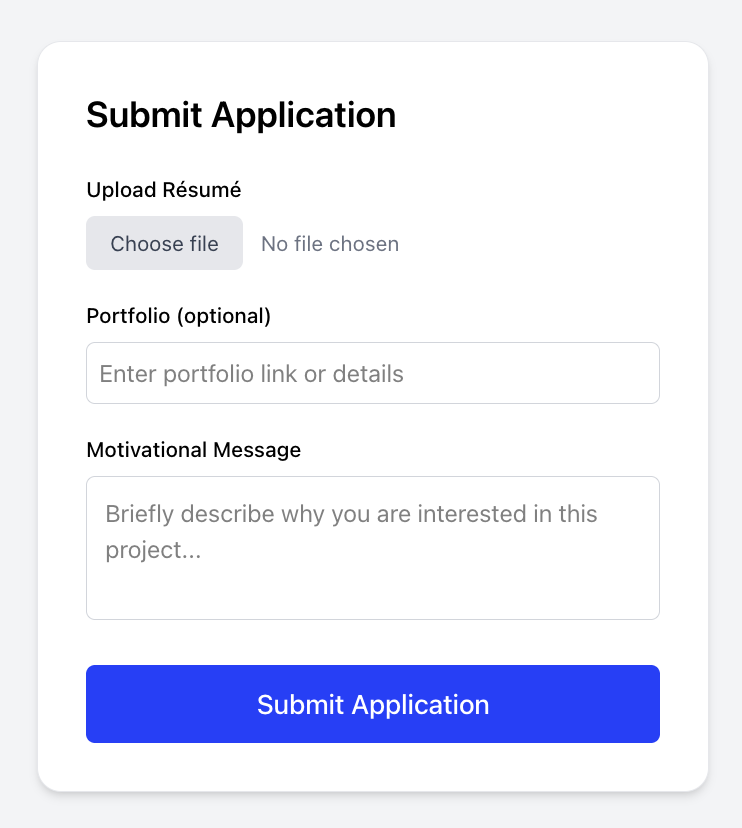
\includegraphics[width=0.85\linewidth]{figures/Student-Submission.png}
  \caption{Student application flow mock-up with guided pitch submission.}
  \label{fig:application-flow}
\end{figure}

I mirror that thought experiment on the organisational journey. Figure~\ref{fig:project-creation} (in Assignment~3) shows the scoping prompts that should keep briefs from arriving half-baked, and the notes imagine automations that alert the founding cohort when new projects drop so acceptance stays quick once the system exists.
